\subsection{Activation}
Doing a LFP analysis of our data, we have the possibility to look at
\textbf{activation} phenomena. They represent how the cerebral cortex reacts to
stimuli, that can be either electrical activities or exogenous stimuli like visual
movements.\\
The simplest way of looking at EEG evoked responses is through \textbf{Event-Related
    Potentials}. When a stimulation is provided to the system, each trial contains a
temporal mixture of signal and noise: signal is likely to be similar across trials,
while noise fluctuates.\\
Thus, it would be better to analyze the data without considering noise. There are
different ways to reduce its impact on the recording - i.e., increase the SNR -:
\begin{itemize}
    \item Averaging the amplitude of the signal across trials (and keeping the time
          dimension), noise cancels out and the ERPs remain.
          \begin{figure}[H]
              \centering
              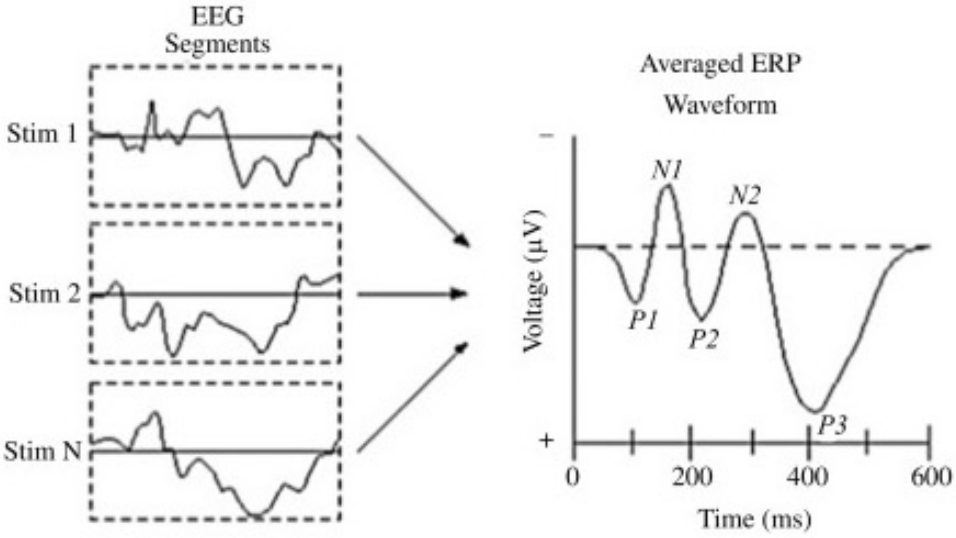
\includegraphics[scale=0.5]{13_1}
          \end{figure}
    \item Another way is to decompose the activity in a joint time-frequency
          representation and then analyze what is the activation in terms of
          time dynamics of the amplitude and how it changes across different frequency
          ranges.
          \begin{figure}[H]
              \centering
              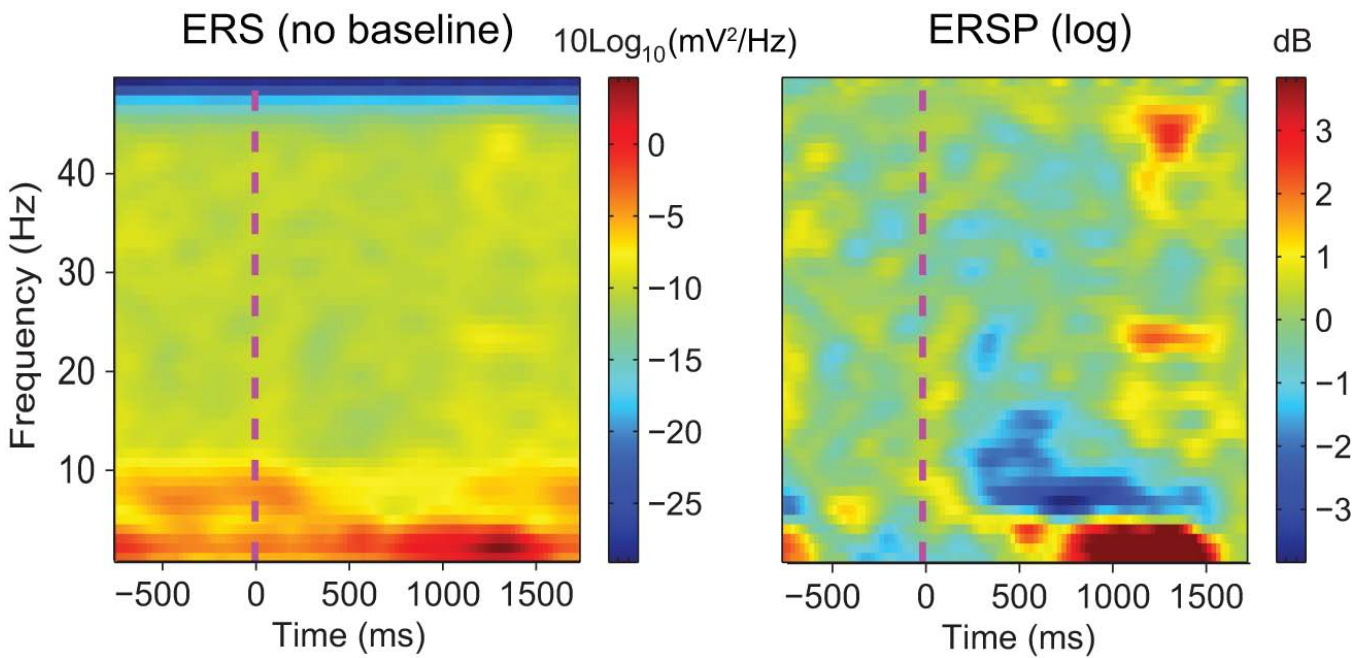
\includegraphics[scale=0.35]{13_2}
          \end{figure}
\end{itemize}
These measures represent amplitude (a.k.a. power) modulations, but what about phase? To
understand the importance of phase let's consider a simple image.
\begin{figure}[H]
    \centering
    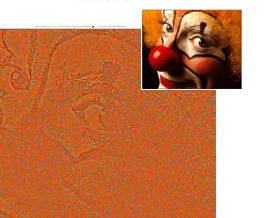
\includegraphics[scale=0.45]{13_3}
\end{figure}
The bigger figure is obtained from the smaller one after randomization of the amplitude
spectrum while keeping the phase spectrum coherent. This means that the spatial
relationship of pixels luminance is contained in the phase rather than in the
amplitude. Therefore, by destroying the amplitude of a signal but keeping the phase
intact still gives the chance to reconstruct much of the information in the data.\\
Hence, considering a 1D signal - i.e., looking at the time variations - the phase
contains the dynamic response of the system more than just the amplitude.
\textbf{Phase coherence} (or synchronization) is a physiological mechanism to promote
communication across the brain network.\\
The capability to separate the phase from the amplitude is important to run analyses
and make inferences.
One possibility to do it is by using the so-called \textbf{Inter-Trial Phase Coherence}
(ITPC) that measures the phase response of a neuronal ensemble given a certain stimulus.
In evoked activity there is the baseline activity and a slow amplitude response (in
some of the channels). An analysis can be realized to understand if the event at some
point triggers a coherent phase response at single sites in the network.
To do it the ERP can be used, but it only finds increases in amplitude - i.e., tells
when the neurons that are below the electrode are synchronized (within the single
event) -. A better option is the ITPC, as it is able to tell when the phase of the
system resets the ongoing oscillations in response to a given stimulus.
Practically speaking, the ITPC is the average across time of the amplitude, but
measured as an average across trials of the phase. The difference with respect to ERPs
is that phase is a radiant value with periodicity, while amplitude is not.
The averaging process is hence realized using the circular statistic properties and
then measuring the resultant factor, which is the length of the vector of the
averaged angles (their values are complex).
\begin{equation*}
    ITPC_{tf}=\biggl|n^{-1}\sum_{r=1}^ne^{ik_{tfr}}\biggr|
\end{equation*}
By computing this term for each time point, a representation of the phase coherence
for every single time point for a given channel across time is finally obtained.
Obviously, for a single time point a lot of angles are present, because a lot of
trials are realized, as can be observed in the following image:
\begin{figure}[H]
    \centering
    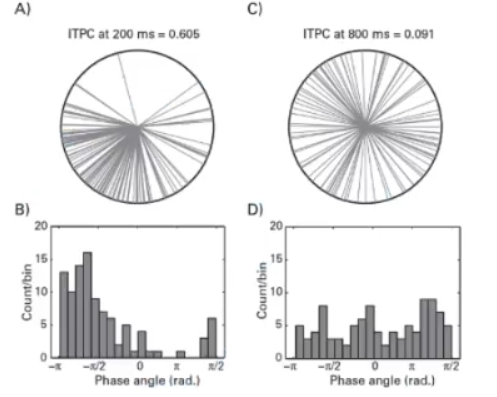
\includegraphics[scale=0.6]{13_4}
\end{figure}
One vector for each trial is plotted and then the resultant is taken: if there is a
preferred phase direction, the resultant vectors are not uniformly distributed on the
unit cycle, while the distribution tends towards this direction.
On the other hand, if there is no causal effect on the event towards the activity,
the phase angles are uniformly distributed on the unit cycle and
the resultant vector will be very small.

\subsection{Connectivity}
Connectivity explains how different brain areas talk to one another and it is based
on a set of methods aimed at quantify interactions between brain regions. There are
three ways to look at and characterize connectivity.
\subsubsection{Structural Connectivity}
\begin{figure}[H]
    \centering
    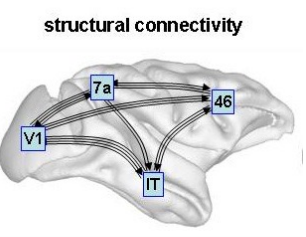
\includegraphics[scale=0.32]{13_5}
\end{figure}
It is the physical link between different brain regions, neurons or neuronal elements,
due to the connections formed by axons one with the other.\\
It is relatively stable at short time scales (seconds or minutes), while at long time
scales (hours or days) it is subject to significant morphological changes and
plasticity.\\
Currently, only invasive tracing studies (cut the brain and the axons) are capable of
demonstrating direct axonal connections. On the other hand, diffusion weighted imaging
techniques, such as DTI, have an insufficient spatial resolution, but they are useful
as whole brain \textit{in vivo} markers of temporal changes in fibers tracts.
\subsubsection{Functional Connectivity}
It is a statistical concept that tells if two regions are likely to share information.
It captures deviations from statistical independence between distributed and often
spatially remote neuronal units, regardless of whether they are connected by direct
structural links or not.\\
It can be estimated in different ways, for instance by measuring the correlation or
the covariance, the spectral coherence or the phase-locking. Often connectivity
matrices showing these kinds of links are built. They are square matrices with the
channels reported on both axes, showing the pairwise connectivity between two of them.
\begin{figure}[H]
    \centering
    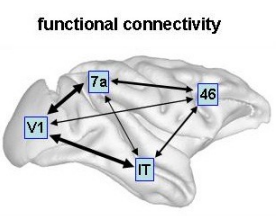
\includegraphics[scale=0.32]{13_6}
\end{figure}
Functional connectivity is highly time-dependent on multiple time scales,
from the short ones to tens of hundreds of milliseconds, but it is not referred to
specific directional effects or to an underlying structural model.
\subsubsection{Effective Connectivity}
\begin{figure}[H]
    \centering
    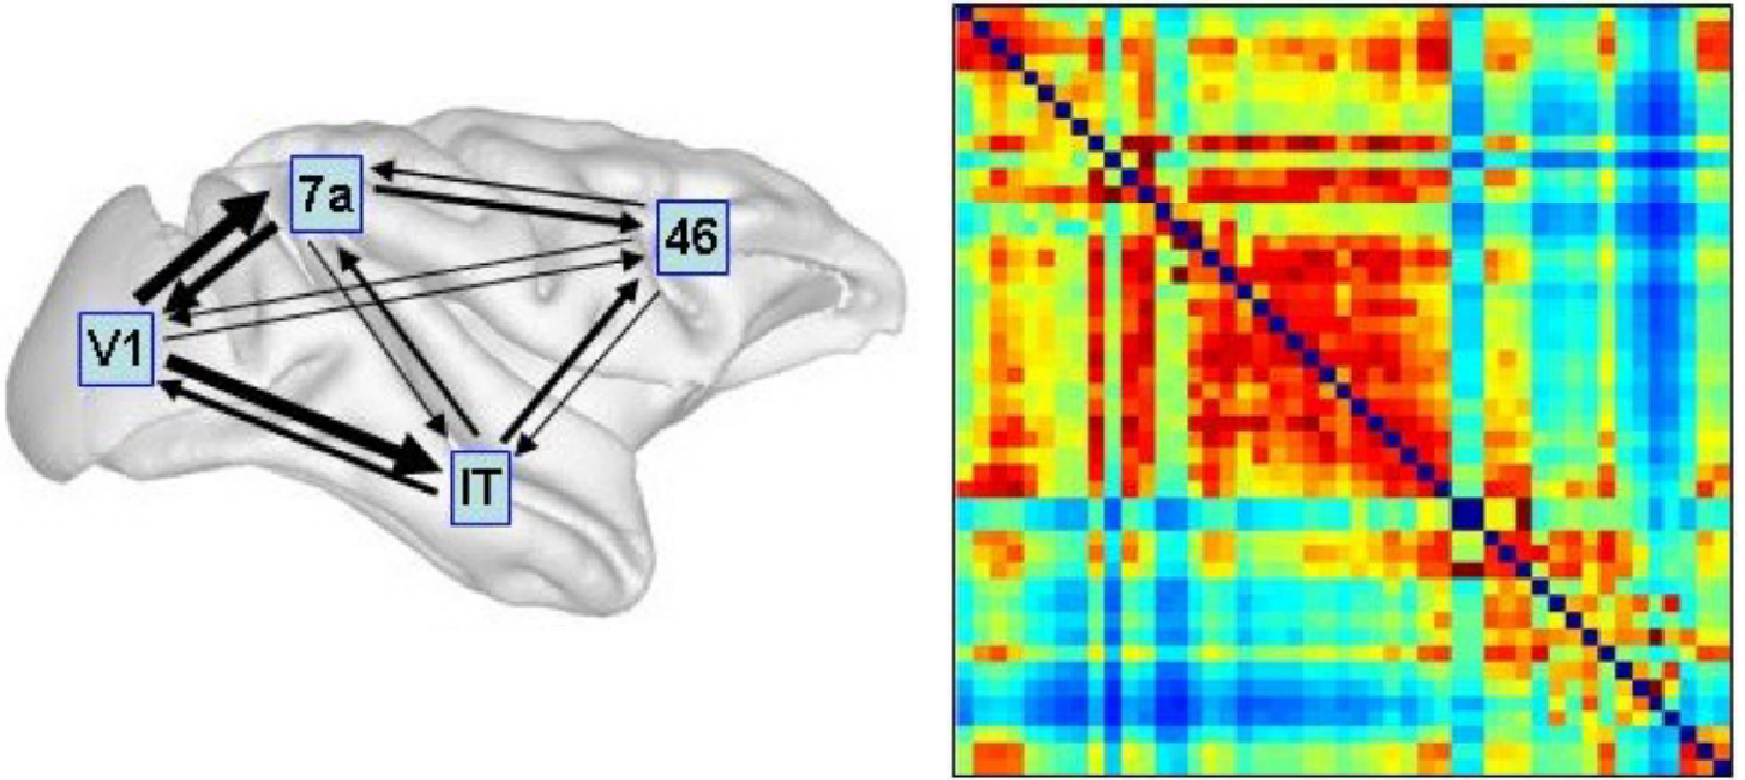
\includegraphics[scale=0.32]{13_7}
\end{figure}
It may be viewed as the union of structural and functional connectivities: it
describes networks of directional and causal effects (it is not a statistical property).
It is generally measured by intervention protocols: causal effects can in fact be
inferred through systematic perturbations of the system or, since causes must precede
effects in time, through time series analysis. One possible way is to look at the
elicited responses across the whole network, given that stimulations are applied to
all the electrodes.
\subsubsection{Integration and Segregation}
\begin{figure}[H]
    \centering
    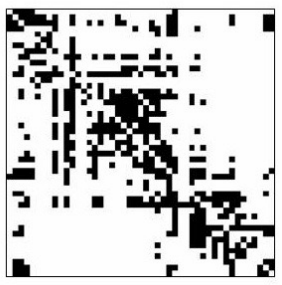
\includegraphics[scale=0.45]{13_8}
\end{figure}
The brain network is fast-evolving in time and slowly-changing in structure connections.
There is a balance in the brain between \textbf{functional integration} and
\textbf{functional segregation}, such that there are regions tightly connected
together and modules where the activity of distinct brain regions is more correlated
are created. These modules contain a single wayout, such wayouts are the \textbf{hubs}
(graph theory). Through these hubs, the single module communicates with other parts of
the network.\\
Connectivity allows to understand which region belongs to which module and which
region is mostly used to communicate between modules.

\subsection{Functional Correlation}
Every analysis related to functional correlation will produce a matrix that shows
the brain is not fully connected, but there are stronger and weaker links.
To study \textit{spontaneous activity} (not the evoked one), some formulations can be
introduced.
\subsubsection{Spectral Coherency}
Spectral coherency is defined as:
\begin{equation*}
    C_{xy} = \frac{s_{xy}(f)}{\sqrt{s_{xx}(f)s_{yy}(f)}}
\end{equation*}
where \(s\) is the Fourier spectrum of the signal.
Spectral coherence is computationally expensive, therefore it is common to down-sample
the data before performing it.\\
Notice that by looking at the connectivity from a spikes-scale point of view,
down-sampling is not possible: the only option is using a sparse matrix.\\
Since \(C_{xy}\) is a complex value, there are two possible ways to look at it:
\begin{itemize}
    \item \textbf{Coherence}:
          \begin{equation*}
              Coh_{xy}=|C_{xy}|
          \end{equation*}
          It is a number comprised between 0 and 1, where 1 means complete coherence and 0
          means no coherence. Of course, 0 never happens. It represents the strenght of the
          connection between the channels.
    \item \textbf{Imaginary Coherence}:
          \begin{equation*}
              iCoh_{xy}=|\Im{C_{xy}}|
          \end{equation*}
          It is important because volume conduction is modelled as zero phase
          synchronization, which only affects the real part of the spectrum. Hence, by
          looking just at the imaginary part the zero lag synchronization can be removed.
\end{itemize}
\subsubsection{Phase Coupling}
A problem of \(C_{xy}\) is that it includes information on both phase synchronization
and amplitude correlation. However, to better analyze either the phase or the
amplitude, the signal can be decomposed using a Morlet transform.\\
From this decomposition, the phase synchronization or \textbf{phase locking value} can
be obtained:
\begin{equation*}
    PLV_{xy}=\biggl|\frac{1}{n}\sum_{t=1}^ne^{j(\phi_x(t)-\phi_y(t)}\biggr|
\end{equation*}
This measure is very similar to the ITPC, even if the PLV is an average across time,
whereas the ITPC is across trials. However, their meaning is the same: if two channels
have a constant time relation (lag), this is reflected in a constant phase difference
measured as the resultant vector of the phase distribution along the unit circle of
all the possible phase angles.\\
Therefore, by looking at the time course there is a high PLV whenever the two
activities are well synchronized, on the contrary, a low PLV is observed for very
different signals across channels.
\begin{figure}[H]
    \centering
    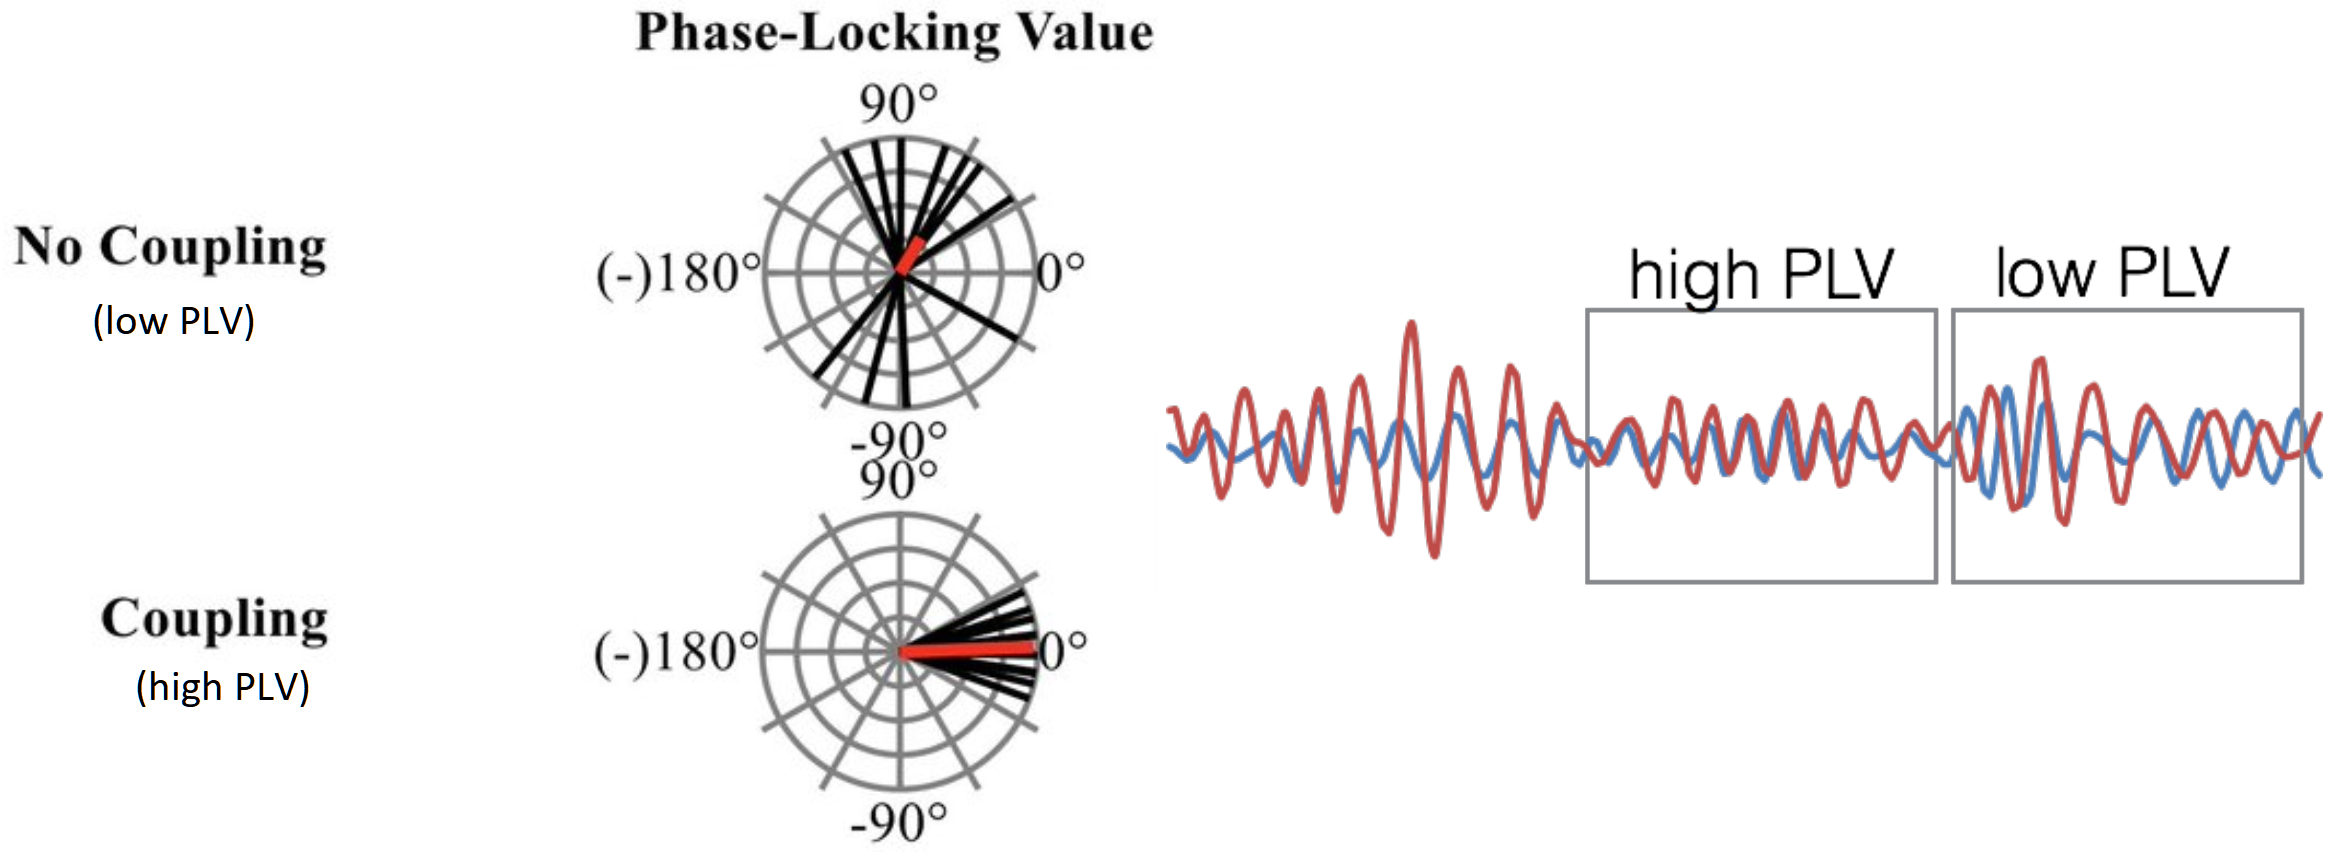
\includegraphics[scale=0.3]{13_12}
\end{figure}
\paragraph{How to assess the significance of coupling?}
At this point, it is important to understand if the obtained results are significant
or not.\\
A classical statistical analysis cannot be done, because every possible measure will
be inflated by an error of type II. Moreover, given that signals are natural, there is
no certainty about which distribution might be used to represent them.\\
Henceforth, a different way should be found. Usually, a \textbf{surrogate approach} is
applied: surrogate data are created, maintaining the auto-correlation of the signals in time,
but breaking down the cross-correlation among the channels. For instance, to test
whether a value obtained using PLV makes sense, a piece of the surrogate data can be
taken, broken into two parts and flipped in the time axis. In this way, the rows of
the surrogate matrix still have the same number of samples, but they are shuffled:
the cross-correlation among channels is disrupted, but the auto-correlation within a
single channel is maintained. This process is then repeated many times.\\
Then, with surrogate distribution a classical hypothesis test can be conducted.
\begin{figure}[H]
    \centering
    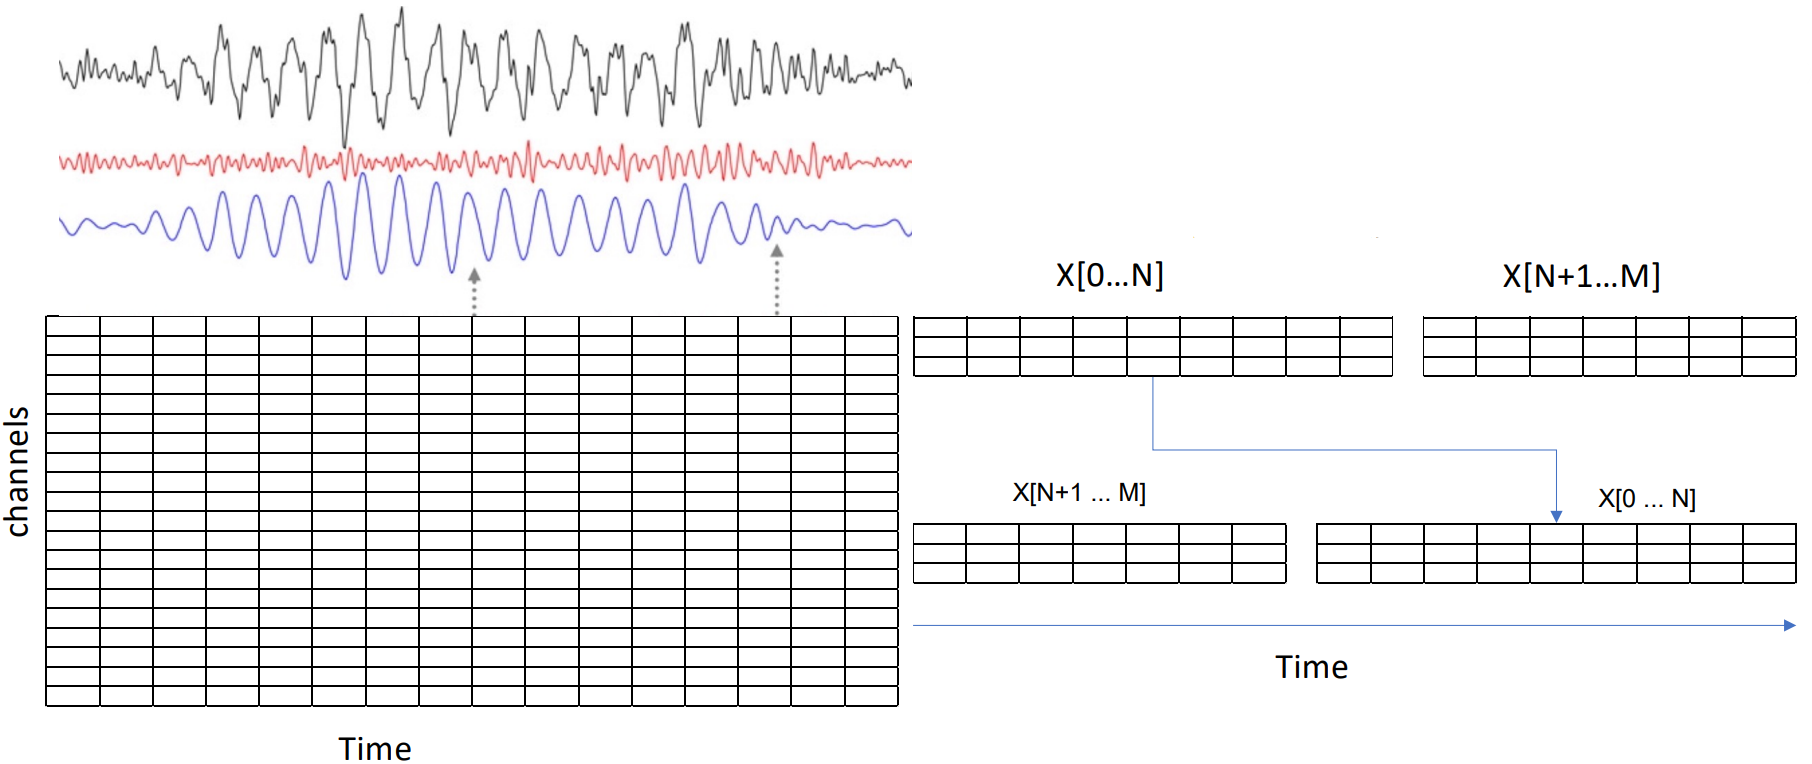
\includegraphics[scale=0.4]{13_13}
\end{figure}
